
\chapter{The Serre Equations}
\label{chp:Serreeqns}

%The Serre equations are partial differential equations that describe the behaviour of waves of free surface flows of fluids for a wide array of wave properties. 

%spectrum of wave models%



%In fact they are considered to be one of the best models for free surface flows up to wave breaking []. For  this reason we are interested in using the Serre equations to model wave hazards such as tsunamis and storm surges. 

%The Serre equations can be derived asymptotically [] or via depth integration [] of the full Navier-Stokes equations. They are evolution type equations, however they are not strictly parabolic or hyperbolic and naively are not in conservation law form.  


% Introduce Serre Equations/ Conservative/ Non-conservative, Non-dimensionalised
% Properties : Conservation of Mass, Energy and Momentum, Dispersion relation, wave speed bounds, Analytic solutions

\section{The Equations}
%[!]-----[!] DISPERSION!!!!!
%full nonlineariy, good approximation to Euler equations up to wave breaking
There are three primary ways in which the Serre equations have been derived from the Euler equations in the past; by asymptotic expansion \cite{Serre-F-1953-857,Bonneton-Lannes-2009-16601}, directed fluid sheets \cite{Green-Naghdi-1976-237} and depth integration \cite{Su-Gardener-1969-536,Zoppou-2014}. In this thesis the depth integration view of the equations is taken, although the derivation is omitted given the extent of literature already available. 

From the depth-integration approach the Serre equations describe a free surface defined by its height $h(x,t)$ above a stationary bed profile $b(x)$ and a depth average of its horizontal velocity $u(x,t)$ as in Figure \ref{fig:WaterModel}. This is the same as the derivation of the Shallow Water Wave Equations (SWWE) [], except for the Serre equations we allow the vertical velocity to vary linearly with depth and so we get non-hydrostatic pressure terms and therefore dispersion.

\begin{figure}
	\centering
	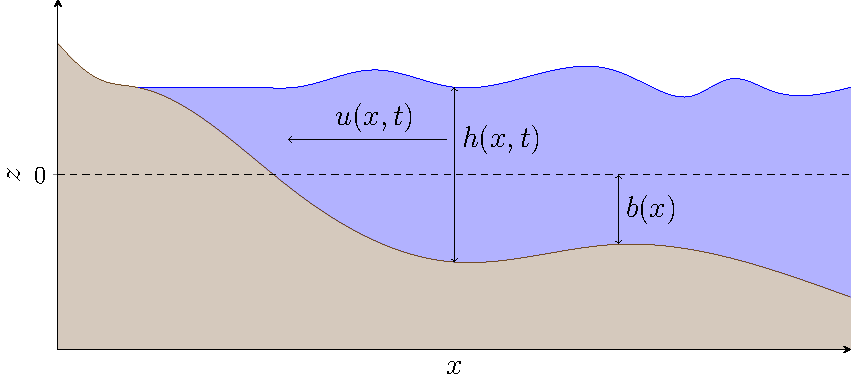
\includegraphics[width=\textwidth]{./chp2/figures/SerreModel.pdf}
	\caption{Diagram demonstrating the quantities used to describe the fluid (\squareF{blue}) and the bed (\squareF{brown!80!black}) for the Serre equations.}
	\label{fig:WaterModel}
\end{figure}

By depth integrating the Euler equations [] with a no-slip condition at the bed and a free surface condition at the free surface we get a depth integrated approximation of the conservation of mass and momentum equations
\begin{subequations}
	\begin{align}
	&\frac{\partial h}{\partial t} + \dfrac{\partial (uh)}{\partial x} = 0,  \label{eqn:FullSerreNonConMass} \\ \nonumber \\
	&\dfrac{\partial (uh)}{\partial t} + \dfrac{\partial}{\partial x} \left ( u^2h + \dfrac{gh^2}{2} + \dfrac{h^2}{2}{\Psi} + \dfrac{h^3}{3}{ \Phi }  \right )  +  \dfrac{\partial b}{\partial x} \left (gh +   h \Psi + \dfrac{h^2}{2}{ \Phi }  \right ) = 0.	\label{eqn:FullSerreNonConMome}
	\end{align}
	\label{eqn:FullSerreNonCon}
\end{subequations}
\begin{defn}
	\label{eqn:FullSerreNonConVarDef}
	The $\Phi$ and $\Psi$ terms account for the non-hydrostatic part of the pressure and are
	\begin{subequations}
	\begin{align}
	{ \Psi }  &= \dfrac{\partial b}{\partial x}\left(\dfrac{\partial u}{\partial t} + u\dfrac{\partial u}{\partial x} \right)  + u^2\dfrac{\partial b}{\partial x}, \label{eqn:SerreeqnPsi} \\
 { \Phi }  &= \dfrac{\partial u }{\partial x} \dfrac{\partial u}{\partial x} -u \dfrac{\partial^2 u}{\partial x^2}  - \dfrac{\partial^2 u}{\partial x \partial t} . \label{eqn:SerreeqnPhi} 
	\end{align}
	\end{subequations}
\end{defn}
When $\Phi = \Psi = 0$ the Serre equations are equivalent to the SWWE where the vertical velocity is constant in depth, only the hydrostatic pressure is present and there is no dispersion of waves. Due to the presence of these $\Phi$ and $\Psi$ terms the Serre equations are much more difficult to solve analytically and numerically than the SWWE. The primary reason for this is that whilst the SWWE are hyperbolic for finite water depth, the Serre equations are neither hyperbolic nor parabolic. Furthermore the Serre equations are not in conservation law form due to the presence of temporal derivatives in $\Phi$ and $\Psi$, although they are derived from conservation equations. 

For a horizontal bed $\partial b / \partial x = 0$, thus $\Psi = 0$ and all the source terms drop out and the Serre equations become
\begin{subequations}
	\label{eqn:FullSerreNonConHorizbed}
	\begin{align}
	\label{eqn:FullSerreNonConMassHorizbed}
	&\frac{\partial h}{\partial t} + \dfrac{\partial (uh)}{\partial x} = 0, \\ \nonumber \\
	\label{eqn:FullSerreNonConMomeHorizbed}
	&\dfrac{\partial (uh)}{\partial t} + \dfrac{\partial}{\partial x} \left ( u^2h + \dfrac{gh^2}{2} + \dfrac{h^3}{3}{ \Phi }  \right ) = 0.
	\end{align}
\end{subequations}	
These equations are still neither hyperbolic nor parabolic and are still not in conservation law from as $\Phi$ contains a temporal derivative. As such even for horizontal beds the Serre equations are more difficult to solve analytically and numerically than the SWWE. 

\subsection{Alternative form of the Serre Equations}
A major hurdle for developing numerical methods for the Serre equations is the presence of the mixed temporal and spatial derivative in $\Phi$ \eqref{eqn:SerreeqnPhi}. By rewriting the Serre  equations and introducing a new conserved quantity $G$ \cite{Hank-etal-2010-2034,Zoppou-2014,Li-2014-169}, the mixed temporal and spatial derivative can be removed and the Serre equations can be written in conservation law form.
\begin{defn}
	\label{defn:SerreEqnConservedQuantity1}
	The conserved quantity $G$ is
	\[ G =  h {u} \left(1 + \frac{\partial h}{\partial x}\frac{\partial b}{\partial x} + \frac{1}{2}h\frac{\partial^2 b}{\partial x^2} + \frac{\partial b}{\partial x}^2 \right) - \frac{\partial}{\partial x}\left(\frac{1}{3}h^3  \frac{\partial {u}}{\partial x}\right).\]
\end{defn}

The Serre equations \eqref{eqn:FullSerreNonCon} are then rewritten as conservation laws for the conserved variables $h$ and $G$
\begin{subequations}
	\label{eqn:FullSerreCon}
	\begin{align}
	& \frac{\partial h}{\partial t} + \dfrac{\partial (uh)}{\partial x} = 0 ,\label{eqn:FullSerreConMass}  \\ \nonumber \\
	\begin{split}
	\label{eqn:Serreconsconmom}
		\frac{\partial G}{\partial t}  + \frac{\partial}{\partial x} \left( {u} G + \frac{gh^2}{2} - \frac{2}{3}h^3 \frac{\partial {u}}{\partial x}^2 + h^2 {u}\frac{\partial {u}}{\partial x}\frac{\partial b}{\partial x} \right) \\ + \frac{1}{2}h^2 {u} \frac{\partial {u}}{\partial x} \frac{\partial^2 b}{\partial x^2}  - h {u}^2\frac{\partial b}{\partial x}\frac{\partial^2 b}{\partial x^2} + gh\frac{\partial b}{\partial x} = 0.
	\end{split}
	\end{align}
\end{subequations}
The conserved quantity $G$ resembles $h$ multiplied by the irrotationality \cite{Choi-Camassa-1999-1,Carter-Cienfuegos-2011-259} and its conservation equation is equivalent to the conservation equation for momentum \eqref{eqn:FullSerreNonConMome}.

This conservation law form makes the Serre equations well suited for a finite volume method for the conservation of mass and $G$ equations, provided one can solve for $u$ given $h$ and $G$. Although this does solve the problem of it not being in conservation law, these equations are still considerably more difficult to solve than the SWWE.

For a horizontal bed $\partial b / \partial x = 0$ the conservation law form of the Serre equations is
\begin{subequations}
	\label{eqn:FullSerreConHorizBed}
	\begin{align}
	&\frac{\partial h}{\partial t} + \dfrac{\partial (uh)}{\partial x} = 0, \label{eqn:FullSerreConMassHorizBed} \\
	&\frac{\partial G}{\partial t}   + \frac{\partial}{\partial x} \left( {u} G + \frac{gh^2}{2} - \frac{2}{3}h^3 \frac{\partial {u}}{\partial x}^2 \right) = 0 , \label{eqn:SerreconsconmomHorizBed}\\
	&G =  h {u}  - \frac{\partial}{\partial x}\left(\frac{1}{3}h^3  \frac{\partial {u}}{\partial x}\right). \label{defn:SerreEqnConservedQuantity1HorizBed}
	\end{align}
\end{subequations}
These equations are much simpler to solve than their counterparts that allow for variations in bathymetry, although they still present a number of challenges.

\section{Properties of the Serre Equations}
The Serre equations are significantly more complex than their dispersionless counterparts the SWWE and so fewer analytic solutions can be found in the literature. This increases the need to utilise the known properties of the Serre equations and construct forced solutions to assess our numerical methods. The relevant properties of the Serre equations are thus presented here, beginning with their conservation properties. 


\subsection{Conservation Properties}
Conservation of a quantity means that in a closed system the total amount of a quantity $q$ remains constant in time.
\begin{defn}
	\label{defn:TotalAmmountab}
	The total amount of a quantity $q$ in a system occurring on the interval $[a,b]$ at time $t$ is
	\begin{equation*}
	\mathcal{C}_q(t) = \int_{a}^{b} q(x,t)\, dx
	\end{equation*}
\end{defn}
Conservation of a quantity $q$ therefore implies that $\mathcal{C}_{q}(0) = \mathcal{C}_{q}(t)$ $\forall t$.

Given that the Serre equations \eqref{eqn:FullSerreNonCon} are conservation equations for mass and momentum and that the conservation of momentum equation can be rewritten as a conservation equation for $G$ \eqref{eqn:FullSerreCon}, the Serre equations conserve these quantities. Additionally owing to the Hamiltonian structure of the Serre equations, the Serre equations possess a Hamiltonian $\mathcal{H}$ which acts as an energy and is therefore also conserved.

\begin{defn}
	\label{eqn:Hamildef}
	The Hamiltonian of the Serre equations is
	\begin{equation*}
		\mathcal{H}(x,t) = \frac{1}{2} \left(hu^2 + \frac{h^3}{3} \left(\frac{\partial u}{\partial x}\right)^2 + gh^2 + 2ghb + u^2h\frac{\partial b}{\partial x} - uh^2 \frac{\partial u}{\partial x} \frac{\partial b}{\partial x}  \right).
	\end{equation*}
\end{defn}
For the system to be closed for the Serre equations the flux terms of the conservation of mass and momentum equations at both boundaries must with cancel each other and the integral of the source terms over the domain must be zero.

\subsection{Dispersion Properties}
The dispersion properties of wave equations are primarily studied through linearising the equations, assuming periodic wave solutions and then deriving a relationship between the frequency $\omega$ and wave number $k$ of these solutions. For the Serre equations the dispersion relation [] is
\begin{equation}
\label{eqn:DispersionRelation}
\omega = Uk \pm k \sqrt{gH} \sqrt{\frac{3}{\left(kH\right)^2 + 3}}.
\end{equation}
\citet{Barthelemy-2004-315} compared this dispersion relation to that of the linear theory of water waves and demonstrated its utility when $k$ is large. However when $k$ is small the difference between the dispersion relation of the Serre equations and that of water wave theory increases, leading to poorer reproduction of experimental observations by the Serre equations. The dispersion relation of the Serre equations can be modified by introducing terms to reduce this difference \cite{Barthelemy-2004-315}, but such modifications are beyond the scope of this thesis.


From the dispersion relation the phase velocity $v_p = \omega / k$  and the group velocity $v_g = \partial \omega / \partial  k$ can be written in terms of wave number as
\begin{subequations}
	\label{eqn:WaveVelocities}
	\begin{equation}
	\label{eqn:WaveVelocitiesPhase}
	v_p = U \pm \sqrt{gH}\sqrt{\frac{3}{\left(kH\right)^2 + 3}},
	\end{equation}
	\begin{equation}
	\label{eqn:WaveVelocitiesGroup}
	v_g = U \pm \sqrt{gH} \left(\sqrt{\frac{3}{\left(kH\right)^2 + 3}} \mp \left(kH\right)^2 \sqrt{\frac{3}{\left(\left(kH\right)^2 + 3 \right)^3}}\right).
	\end{equation}
\end{subequations}
Since both the phase and group velocities depend on the wave number, waves of different spatial frequencies travel at different speeds meaning the Serre equations describe dispersive waves.

Fortunately, the phase velocity and the group velocity of waves are bounded, since as $k \rightarrow 0$ then $v_p,v_g \rightarrow U$ and as $k \rightarrow \infty$ then $v_p,v_g \rightarrow U \pm \sqrt{gH}$. Therefore we have that
\begin{subequations}
\begin{align}
&U - \sqrt{gH} \le v_p \le U + \sqrt{gH}, \label{eqn:WaveVelocitiesBound} \\
&U - \sqrt{gH} \le v_g \le U + \sqrt{gH}.
\end{align}
\end{subequations}

\subsection{Analytic Solutions}
Due to the complexity of the Serre equations, few analytic solutions have been discovered. In particular there is a travelling wave solution for horizontal beds and a lake at rest solution for any bathymetry. Both analytic solutions will be used to assess the capabilities of the numerical methods and so we present them here. 

\subsubsection{Solitary Travelling Wave Solution}
The Serre equations admit a travelling wave solution that propagates at a constant speed without deformation due to a balance between nonlinear and dispersive effects. Unlike the Euler equations this travelling wave solution has a closed form
\begin{subequations}
	\begin{align}
	&h(x,t) = a_0 + a_1\text{sech}\left(\kappa \left(x - ct\right)\right), \\
	&u(x,t) = c\left(1 - \dfrac{a_0}{h(x,t)}\right), \\
	&b(x) = 0
	\end{align}
	\label{eqn:Solitondefhub}
\end{subequations}
with
\begin{align*}
&\kappa = \dfrac{\sqrt{3a_1}}{2 a_0\sqrt{\left(a_0 + a_1\right)}}, \\ \\
&c = \sqrt{g(a_0 + a_1)}.
\end{align*}

This wave is has an amplitude of $a_1$, an infinite wavelength and propagates on water $a_0$ deep. These solitary waves are not true solitons however, due to their inelastic collisions with one another \cite{Dutykh-etal-2013-761}. These solitary waves can also be generalised to a family of periodic solutions \cite{El-etal-2006} which are all periodic travelling wave solutions. 

From \eqref{eqn:Solitondefhub} we can derive $G$ for the solitary wave solution in terms of $h$
\begin{equation}
G =c(h - a0) - \frac{ca_0}{3} \left(h\frac{\partial^2 h}{\partial x^2 } + \left[\frac{\partial h}{\partial x }\right] \right)
\label{eqn:SolitondefG}
\end{equation}
where the derivatives of $h$ are
\begin{align*}
&\frac{\partial h}{\partial x } = -2 a_1 \kappa \text{sech}^2\left(\kappa \left(x - ct\right)\right) \text{tanh}\left(\kappa \left(x - ct\right)\right),\\
&\frac{\partial^2 h}{\partial x^2 } =  2a_1 \kappa^2 \left(\text{cosh}\left(2\kappa \left(x - ct\right)\right) -2\right)\text{sech}^4\left(\kappa \left(x - ct\right)\right).
\end{align*}

As we would like to assess the conservation properties of our numerical methods we will require the total mass, momentum, $G$ and Hamiltonian for this solution. In particular we require these totals at the initial time $t=0$, to allow for various domains we present the integrals in indefinite form 
\begin{subequations}
	\begin{align}
	\int h(x,0) \; dx = {} & a_0 x + \frac{a_1}{\kappa} \tanh\left(\kappa x\right) + \text{constant}, \\
	\int u(x,0)h(x,0) \;  dx = {} & \frac{a_1 c}{\kappa} \tanh\left(\kappa x\right)+ \text{constant}, \\
	\begin{split}
	\int G(x,0) \; dx = {}&  \frac{c a_1}{3 \kappa}  \Bigg(3 + 2a_0^2 \kappa^2\text{sech}^2\left(\kappa x\right)  \\ &+ 2a_0 a_1 \kappa^2 \text{sech}^4\left(\kappa x\right) \Bigg)\tanh\left(\kappa x\right)  + \text{constant} ,
	\end{split}
	\\
	\begin{split}
	\int \mathcal{H}(x,0) \; dx = {}&\frac{1}{2} \Bigg(\int g\left[h(x,0)\right]^2 \; dx + \int h(x,0)\left[u(x,0)\right]^2 \; dx  \\ &+ \int \left[h(x,0)\right]^3 \left[\frac{\partial u(x,0)}{\partial x}\right]^2 \; dx \Bigg) 
	\end{split}
	\end{align}
	\label{eqn:SolitonConservation}
\end{subequations}

where the integrals of the Hamiltonian are

\begin{align*}
\begin{split}
\int g\left[h(x,0)\right]^2 \; dx ={}& \frac{g}{12 \kappa }\text{sech}^3\left(\kappa x\right) \Bigg[9a_0^2 \kappa x \cosh\left(\kappa x\right) + 3 a_0^2 \kappa x \cosh\left(3\kappa x\right) \\ &+ 4 a_1 \left(3a_0 + 2 a_1 + \left(3a_0 + a_1\right)\cosh\left(2\kappa x\right)\right) \sinh\left(\kappa x\right)\Bigg] \\ &+ \text{constant},
\end{split}\\ \\
\begin{split}
\int h(x,0)\left[u(x,0)\right]^2 \; dx = {}& \frac{\sqrt{a_1}c^2}{\kappa} \Bigg( -\frac{a0}{\sqrt{a_0 + a_1}} \text{arctanh}\left(\dfrac{\sqrt{a1} \tanh\left(\kappa x\right)}{\sqrt{a_0 + a1}}\right)\\ &+ \frac{\sqrt{a_1}}{\kappa}\tanh\left(\kappa x\right)\Bigg)  + \text{constant},
\end{split} 
\\ \\
\begin{split}
\int \left[h(x,0)\right]^3 \left[\frac{\partial u(x,0)}{\partial x}\right]^2 \; dx = {}& \frac{2a_0^2c^2 \kappa }{9 \sqrt{a_1} \left(a_0 + a_1\text{sech}^2\left(\kappa x \right) \right)}   \\ &\times\left(a_0 + 2a_1 + a_0 \cosh\left(2\kappa x\right) \right) \text{sech}^2\left(\kappa x\right) \\&\times \Bigg[-3 a_0 \sqrt{a_0 + a_1}\text{arctanh}\left(\dfrac{\sqrt{a1} \tanh\left(\kappa x\right)}{\sqrt{a_0 + a1}}\right)  \\ &+ \sqrt{a_1}\left(3a_0 + a_1 - a_1\text{sech}^2\left(\kappa x\right)\right)\tanh(\kappa x) \Bigg]+ \text{constant}.
\end{split}
\end{align*}

Therefore, we have the analytic values of our physical variables $h$, $u$, $G$ and $b$ for all $t$ as well as the total amounts of our conserved quantities for the initial conditions when $t=0s$ as desired.

\subsubsection{Lake at Rest}
The lake at rest solution is a rudimentary stationary solution of the Serre equations that exists for all bathymetry $b(x)$ and is defined by
\begin{subequations}
	\begin{align}
	&h(x,t) = \max\left\lbrace a_0 - b(x), 0 \right\rbrace, \\
	&u(x,t) = 0 , \\
	&G(x,t) = 0 .
	\end{align}
	\label{eqn:LARdefhub}
\end{subequations}
It represents a quiescent body of water with a horizontal water surface or stage $w(x,t) = h(x,t) + b(x)$ over any bathymetry. The maximum function is included for the water depth to allow for dry regions of the bed when $b(x) > a_0$. We write these solutions in terms of $b(x)$ as this solution holds for all bed profiles. 

For these quantities \eqref{eqn:LARdefhub} the Serre equations \eqref{eqn:FullSerreCon} reduce to
\begin{align*}
& \frac{\partial h}{\partial t}  = 0 , \\
&\frac{\partial G}{\partial t}  +\dfrac{\partial}{\partial x} \left(\frac{gh^2}{2}\right) + gh \frac{\partial b}{\partial x} = 0.
\end{align*}
Since we have that $\partial h / \partial x =  - \partial b / \partial x$ when $h \neq 0$, then $G$ and $h$ are constant in time and therefore so is $u$ and thus we possess a stationary solution of a lake at rest. 
  
The total momentum and $G$ in our system is straightforward to calculate as both are zero everywhere and so we have 
\begin{align}
&\int u(x,0)h(x,0) \;  dx = {} 0 + \text{constant}, \\
&\int G(x,0) \; dx = {} 0 + \text{constant}.
\end{align}
To calculate the total mass and Hamiltonian in our system we must break up our domain into wet regions where $b(x) < a_0$ and dry regions where $b(x) \ge a_0$. For the dry regions the total mass and energy are $0$ and so we have 
 \begin{subequations}
 	\begin{align}
 	\int h(x,0) \; dx = {} & 0 , \\
 	\int \mathcal{H}(x,0) \; dx = {} & 0
 	\end{align}
 \end{subequations}
 whilst in a wet region we have 
 
  \begin{subequations}
  	\begin{align}
  	\int h(x,0) \; dx = {} & a_0 x -  \int b(x) \; dx , \\
  	\int \mathcal{H}(x,0) \; dx = {} & \frac{g}{2} \left(a_0^2x  -  2a_0 \int b(x) \; dx + \int b(x)^2 \; dx \right).
  	\end{align}
  \end{subequations}
  
Therefore as desired we have expressions for all the quantities in terms of the bed profile $b(x)$. 


\subsection{Forced Solutions}
%Gaussian
To account for the small number of analytic solutions to the Serre equations we also constructed forced solutions to assess our numerical methods. These work by introducing a source term $S$ for both the conservation of mass and  momentum (or $G$) equations that balances these equation to force a solution. So for instance we add the source terms $S_{\text{mass}}$ and $S_{G}$ into \eqref{eqn:FullSerreCon} so that we have


\begin{subequations}
	\label{eqn:FullSerreConForced}
	\begin{align}
	& \frac{\partial h}{\partial t} + \dfrac{\partial (uh)}{\partial x} + S_{\text{mass}}  = 0 ,\label{eqn:FullSerreConMassForced}  \\ \nonumber \\
	\begin{split}
	\label{eqn:SerreconsconmomForced}
	\frac{\partial G}{\partial t}  + \frac{\partial}{\partial x} \left( {u} G + \frac{gh^2}{2} - \frac{2}{3}h^3 \frac{\partial {u}}{\partial x}^2 + h^2 {u}\frac{\partial {u}}{\partial x}\frac{\partial b}{\partial x} \right) \\ + \frac{1}{2}h^2 {u} \frac{\partial {u}}{\partial x} \frac{\partial^2 b}{\partial x^2}  - h {u}^2\frac{\partial b}{\partial x}\frac{\partial^2 b}{\partial x^2} + gh\frac{\partial b}{\partial x} + S_{G} = 0.
	\end{split}
	\end{align}
\end{subequations}

as our new forced Serre equations in conservation law form. To construct the forced solution we choose some functions for $h$, $u$ and $b$ for all $x$ and $t$, which will be our forced analytic solutions to the forced Serre equations. From these chosen functions we determine $G$, $S_{\text{mass}}$ and $S_{G}$ so that these equations \eqref{eqn:FullSerreConForced} possess our chosen $h$, $u$ and $b$ as solutions.

We demonstrate this for the particular forced function we employ, a travelling Gaussian wave over a periodic bed profile which has
\begin{subequations}
	\begin{align}
	&h(x,t) = a_0 + a_1\exp\left(-\dfrac{ \left(\left(x - a_2t\right) - a_3 \right)^2}{2a_4}\right), \\
	&u(x,t) = a_5\exp\left(-\dfrac{ \left(\left(x - a_2t\right) - a_3 \right)^2}{2a_4}\right), \\
	&b(x) = a_6\sin\left(a_7 x\right).
	\end{align}
	\label{eqn:SerreGaussBumpPeriodic}
\end{subequations}
From these definitions $G$ can be calculated using Def \ref{defn:SerreEqnConservedQuantity1} while $S_{\text{mass}}$ and $S_{G}$ can be calculated using 
\begin{align*}
&  S_{\text{mass}} = -\frac{\partial h}{\partial t} - \dfrac{\partial (uh)}{\partial x} ,  \\ \nonumber \\
\begin{split}
S_{G} = -\frac{\partial G}{\partial t}  - \frac{\partial}{\partial x} \left( {u} G + \frac{gh^2}{2} - \frac{2}{3}h^3 \frac{\partial {u}}{\partial x}^2 + h^2 {u}\frac{\partial {u}}{\partial x}\frac{\partial b}{\partial x} \right) \\ - \frac{1}{2}h^2 {u} \frac{\partial {u}}{\partial x} \frac{\partial^2 b}{\partial x^2}  + h {u}^2\frac{\partial b}{\partial x}\frac{\partial^2 b}{\partial x^2} - gh\frac{\partial b}{\partial x}
\end{split}
\end{align*}
with $h$, $u$ and $b$ from \eqref{eqn:SerreGaussBumpPeriodic} and the corresponding $G$.

With these values the forced Serre equations \eqref{eqn:FullSerreConForced} admit the analytic solutions \eqref{eqn:SerreGaussBumpPeriodic}. This allows us to assess our numerical solutions for a larger range of scenarios than possible with the current analytic solutions of the Serre equations.


\subsection{Asymptotic Results}
Beyond analytic solutions to the Serre equations there has also been studies of the long term behaviour of the Serre equations for situations that are difficult to treat analytically. One particular scenario of interest is the evolution of a moving discontinuous jump in $h$ known as a bore, which can be observed naturally, for example tidal bores []. There is an analytic solution for bores for the SWWE, but not for the Serre equations.

To gain some insight into the behaviour Whitham modulation techniques were applied to the Serre equations to study the behaviour of bores of the Serre equations as $t \rightarrow \infty$ \cite{El-etal-2006}. These techniques provided an estimate of the speed $S^+$ and amplitude $A^+$ of the front of a bore

\begin{subequations}
	\begin{align}
	&\frac{\Delta}{\left(A^+ + 1\right)^{1/4}} - \left(\frac{3}{4 -  \sqrt{A^+ + 1}}\right)^{21/10} \left(\frac{2}{1 + \sqrt{A^+ + 1}}\right)^{2/5} = 0	\label{eqn:Aplusdef} \\
	&S^+ = \sqrt{g \left(A^+ + 1\right)}	\label{eqn:Splusdef}
	\end{align}
	\label{eqn:ELWhitMod}	
\end{subequations}
where $\Delta = h_b / h_0$, $h_b$ is the height of the bore and $h_0$ is the depth of still water in front of the bore. These estimates were demonstrated to agree well with numerical simulations provided that $\Delta < 1.43$ \cite{El-etal-2006}.